%! Author = smen851
%! Date = 11/07/2024

% Preamble

\documentclass[11pt, a4paper]{scrartcl}

% Packages


\usepackage[utf8]{inputenc}

\usepackage{pgfplots}
\usepackage{amsmath}
% lorem package is used to generate random text for testing
\usepackage{lipsum}
\usepackage{bold-extra}
\usepackage{geometry}
\usepackage{subfigure}
\usepackage{import}
\usepackage{graphicx}
\usepackage{layouts}
\usepackage{caption}
\captionsetup[figure]{name={Fig.}}
\usepackage[section]{placeins}
\usepackage{hyperref}
\usepackage{placeins}


\geometry{a4paper, total={170mm,257mm}, left=25mm, right=25mm, top=10mm, bottom=25mm}
%%Macros
\graphicspath{ {../src/figures/} }
\newcommand{\sect}[1]{Section~\ref{#1}}
\newcommand{\degrees}{\ensuremath{^\circ}}
\renewcommand{\figurename}{Fig.}
% workaround for pgfplots
\def\mathdefault#1{#1}


% Title
\title{Dynamic Antenna Pattern and SAR Performances: \\Notes on Methods and Implementation}
\author{\texttt{Simone Mencarelli}}
\date{\small{\texttt{July 2024}}}
% Document
\begin{document}
    \maketitle


    \section{Antenna Model}
    \label{sec:antenna_model}
    Assuming the SAR antenna is a \emph{ReflectArray}~(RA), e.g., like the JPL radar~\cite{swot}.
    The conformal surface (of the deployable structure) is modeled as an array of \emph{atomic} re-readiating elements.
    For the purpose of this model the implementation of the atomic element is not relevant, and we will be concerned only
    with the surface impedance properties of each cell.
    Summarizing~\cite{MetaTutorialLiu2023}, with a variable local reactive surface impedance, the reflection pattern can
    be shaped and steered in directions different from the specular one.
    This property of RA (and generally of meta-surfaces) is called \emph{anomalous reflection} and can be used, for example, to approximate the reflection properties
    of a parabolic reflector using a flat surface~\cite{rapozar}; or to shape the far field pattern~\cite{Guarrielllo} of a reflector antenna.
    In practice, the surface impedance modulation, is obtained varying some physical parameters of the atomic element
    like a printed patch size, or the distance and thickness of a series of printed concentric rings or squared rings;
    or again, any structure exhibiting some sort of resonant behavior.
    Examples in literature relevant to flown or hypothetical space missions include elements of the square patch
    type~\cite{swot,marco,isara}, or phoenix cells~\cite{Guarrielllo,secondphoenix}.
    The latter exibiting a \emph{phoenix rebirth} property, meaning that the shape of the elements is similar for
    relative small reflection phase--shift differences also at the 2$\pi$--0 transition in a circular fashion.
    Moreover, phoenix cells offer more degrees of freedom, possibly allowing for better optimization opportunities.
    Other RA cells with a high number of degrees of freedom are possible exploiting complex geometries or multi-layer structures
    to improve specific aspects like the cross--polarization reflection coefficient, e.g.~\cite{PradoCrosspolar2017}.
    RA are, in general, designed under the so-called \emph{Local Periodicity Approximation} (LPA), i.e., the individual
    atoms reflection properties are characterised in the specular reflection direction assuming a periodic surface made
    of identical elements; it follows that the spatial sampling of the surface has to be smaller or equal to half a
    wavelength ($\lambda/2$) to avoid multimodal reflections~\cite{MetaTutorialLiu2023}.
    When modulating (and truncating) the surface impedance of the reflector, in practice, the periodicity is broken and multiple
    reflection mechanisms are allowed~\cite{Esposti2022,NayeriRAbook}.
    It is difficult, however, to predict the exact multi-modal reflection pattern unless a full-wave simulation is
    performed which might be very time and memory--consuming for such electrically large structures.
    For this reason, the classical design approach involves designing the RA cells under the LPA and then validating the
    design with a full-wave simulation or measurements~\cite{NayeriRAbook,rapozar,PradoDatabase2022}.
    To control unwanted reflections, the reflector is illuminated with some taper towards the edges to reduce the contribution
    of edge diffraction and the aperiodicity caused by fast-varying impedance profiles~\cite{NayeriRAbook}.
    To understand the effects of mechanical deformations on the antenna pattern, only the anomalous reflection
    is considered assuming an ideal RA with lossless phase--shifting elements.
    Furthermore, especially for a large reflector with small f/D ratios, the anomalous reflection will be
    particularly sensitive to shape variations of the surface due to the relative added phase-delay.
    Also, it makes sense to consider a uniform illumination of the reflecting surface to account for the worst-case scenario
    and fully characterise the effects of any deformation.
    The physical-optics model to compute the (anomalous reflection component of the) antenna pattern is described in~\sect{subsec:physical_optics_conformal_reflectarray_model}.
    The deformation model and the resulting patterns are described in~\sect{subsec:deformation_model}.
    Some considerations on the symmetries of the antenna pattern, to reduce the computation time, are given in~\sect{subsec:symmetries}.

    \subsection{Physical-Optics Conformal Reflectarray Model}
    \label{subsec:physical_optics_conformal_reflectarray_model}
    The integration procedure is the same of~\cite{PradoCrosspolar2017}.\\
    In short:\\
    \noindent\rule{\textwidth}{0.4pt}
    \begin{ttfamily}
        \small
        Assuming every cell is a $\lambda/2$ square uniform aperture:
        \begin{enumerate}
            \item Compute Tangential E-field illumination.
            \item \textbf{For} every cell:
            \begin{enumerate}
                \item Compute $\mathbf{E}_{r}^{x,y} = \mathbf{\sigma} \mathbf{E}_{i}^{x,y}$.
                \item Compute Reflected field $\mathbf{E}_{r}$-$\mathbf{H}_{r}$ (elements LCS):\\
                $\mathbf{E}_{r} \cdot \mathbf{k} = 0$ ; $\mathbf{H}_{r} = \frac{(\mathbf{k} \times \mathbf{E}_{r})}{\eta}$.
                \item Compute element pattern assuming magnetic and electric current \\excitations:
                ${E}_{r}^{x,y}$ and ${H}_{r}^{x,y}$.
            \end{enumerate}
            \item Conformal Array summation (elemental pattern rotation, displacement and sum).
        \end{enumerate}
    \end{ttfamily}
    * to be expanded *\\
    \noindent\rule{\textwidth}{0.4pt}


    \begin{figure}[!tb]
        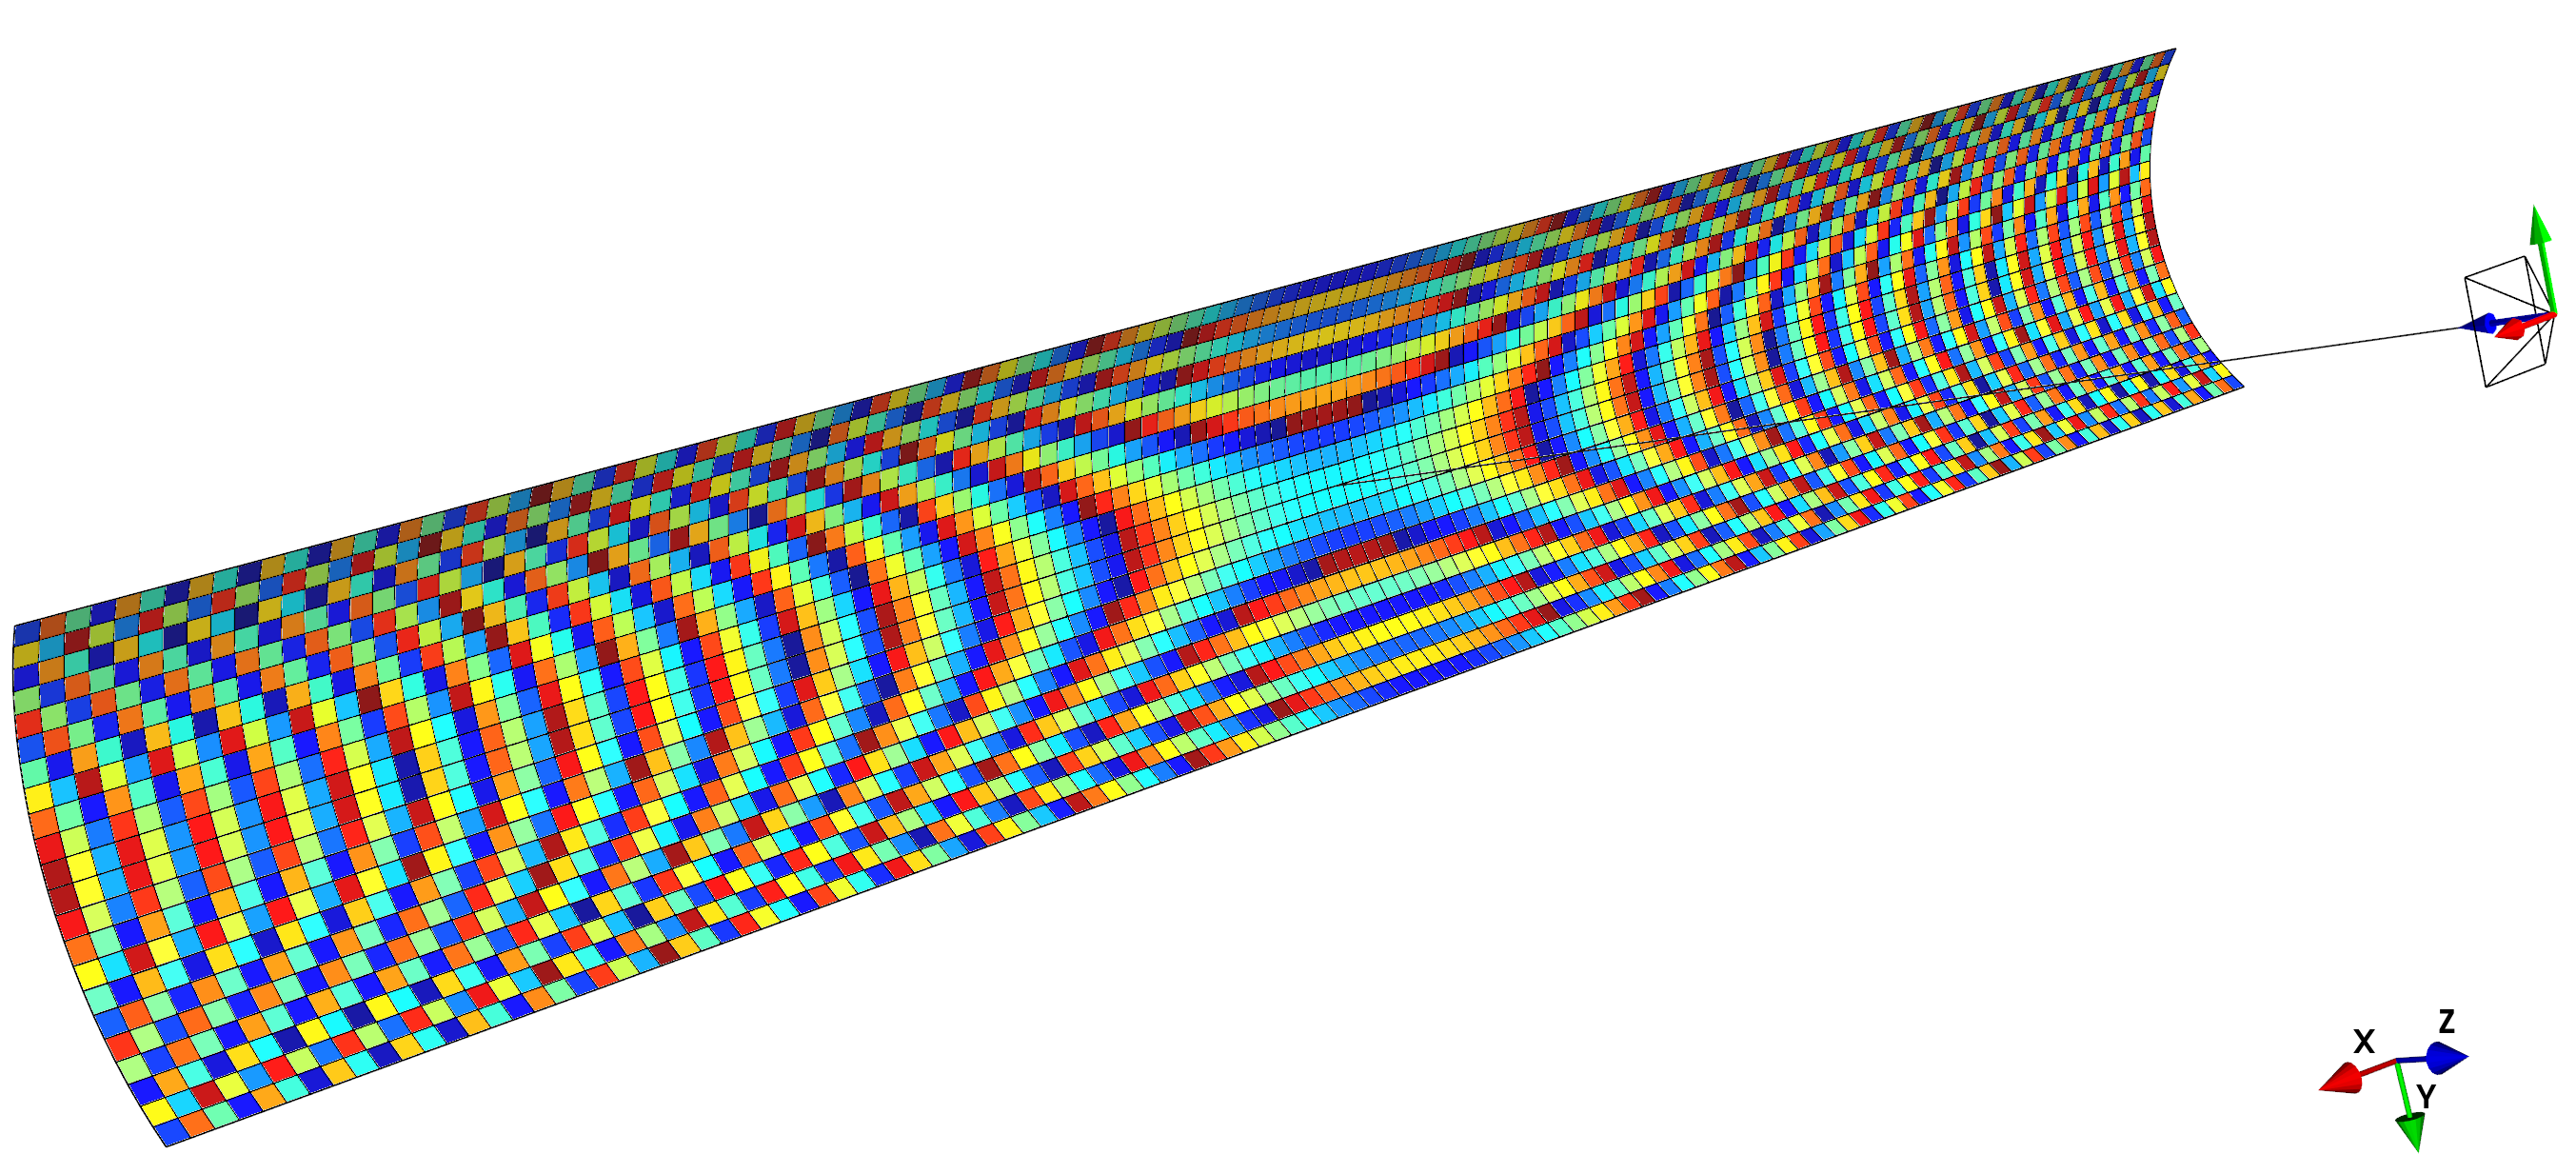
\includegraphics[width=\textwidth]{rageometry}
        \caption{Reflectarray geometry and required phase shift for broadside ($\mathbf{\hat{z}}$) collimation.
        The feed is suspended 1 m above the reflector center; the overall size for the reflector is 2~m in
        length and 0.3~m in width, the surface is cylindrical with cross--section corresponding to a 90\degrees
        subtended angle.}
        \label{fig:rageom}
    \end{figure}

    \begin{figure}[!hbt]
        \centering
        \import{./figures}{linear_pattern.pgf}
        \caption{Far-field pattern for uniformly illuminated reflectarray in the nominal state.
        Elevation coordinate limited to~$\theta \in [0,20]$\degrees
        }
        \label{fig:pattern}
    \end{figure}

    \subsection{Deformation And Dynamic Antenna Pattern}
    \label{subsec:deformation_model}
    The deformation vector is retrieved from the mechanical modal analysis and scaled according to the deformation state
    identified by the oscillation phase $\varphi$ and the maximum amplitude.
    Cell origin deformation vector is computed as the average of the deformation vectors of the four corners of the cell.
    The position of each reflectarray cell is then shifted by summing the averaged deformation vector and rotated
    according to an ortho-normal basis, obtained by averaging and Gram-Schmidt orthogonalization of the deformed mesh
    cell edge vectors (the mechanical simulation mesh uses 4-points cells already the size of a RA atom).
    The far field is recomputed as in~\sect{subsec:physical_optics_conformal_reflectarray_model} with the updated cell
    positions, keeping the same surface impedance profile $\mathbf{\sigma}$ required for collimation in the nominal state.

    \begin{figure}[!hbt]

        \begin{subfigure}
            \centering
            \import{./figures}{deform_pattern_neg.pgf}
            \caption{Far-field pattern for uniformly illuminated reflectarray in the extreme deformed state (negative deformation), i.e.,
                amplitude scaling~=~1, oscillation phase~=~--90\degrees.
                Elevation coordinate limited to~$\theta \in [0,20]$\degrees}
            \label{fig:deformpatternneg}
        \end{subfigure}

        \begin{subfigure}
            \centering
            \import{./figures}{deform_pattern.pgf}
            \caption{Far-field pattern for uniformly illuminated reflectarray in the extreme deformed state, i.e.,
                amplitude scaling~=~1, oscillation phase~=~90\degrees.
                Elevation coordinate limited to~$\theta \in [0,20]$\degrees}
            \label{fig:deformpattern}
        \end{subfigure}
    \end{figure}

    \subsection{Symmetries}
    \label{subsec:symmetries}
    \begin{figure}[!hbt]
        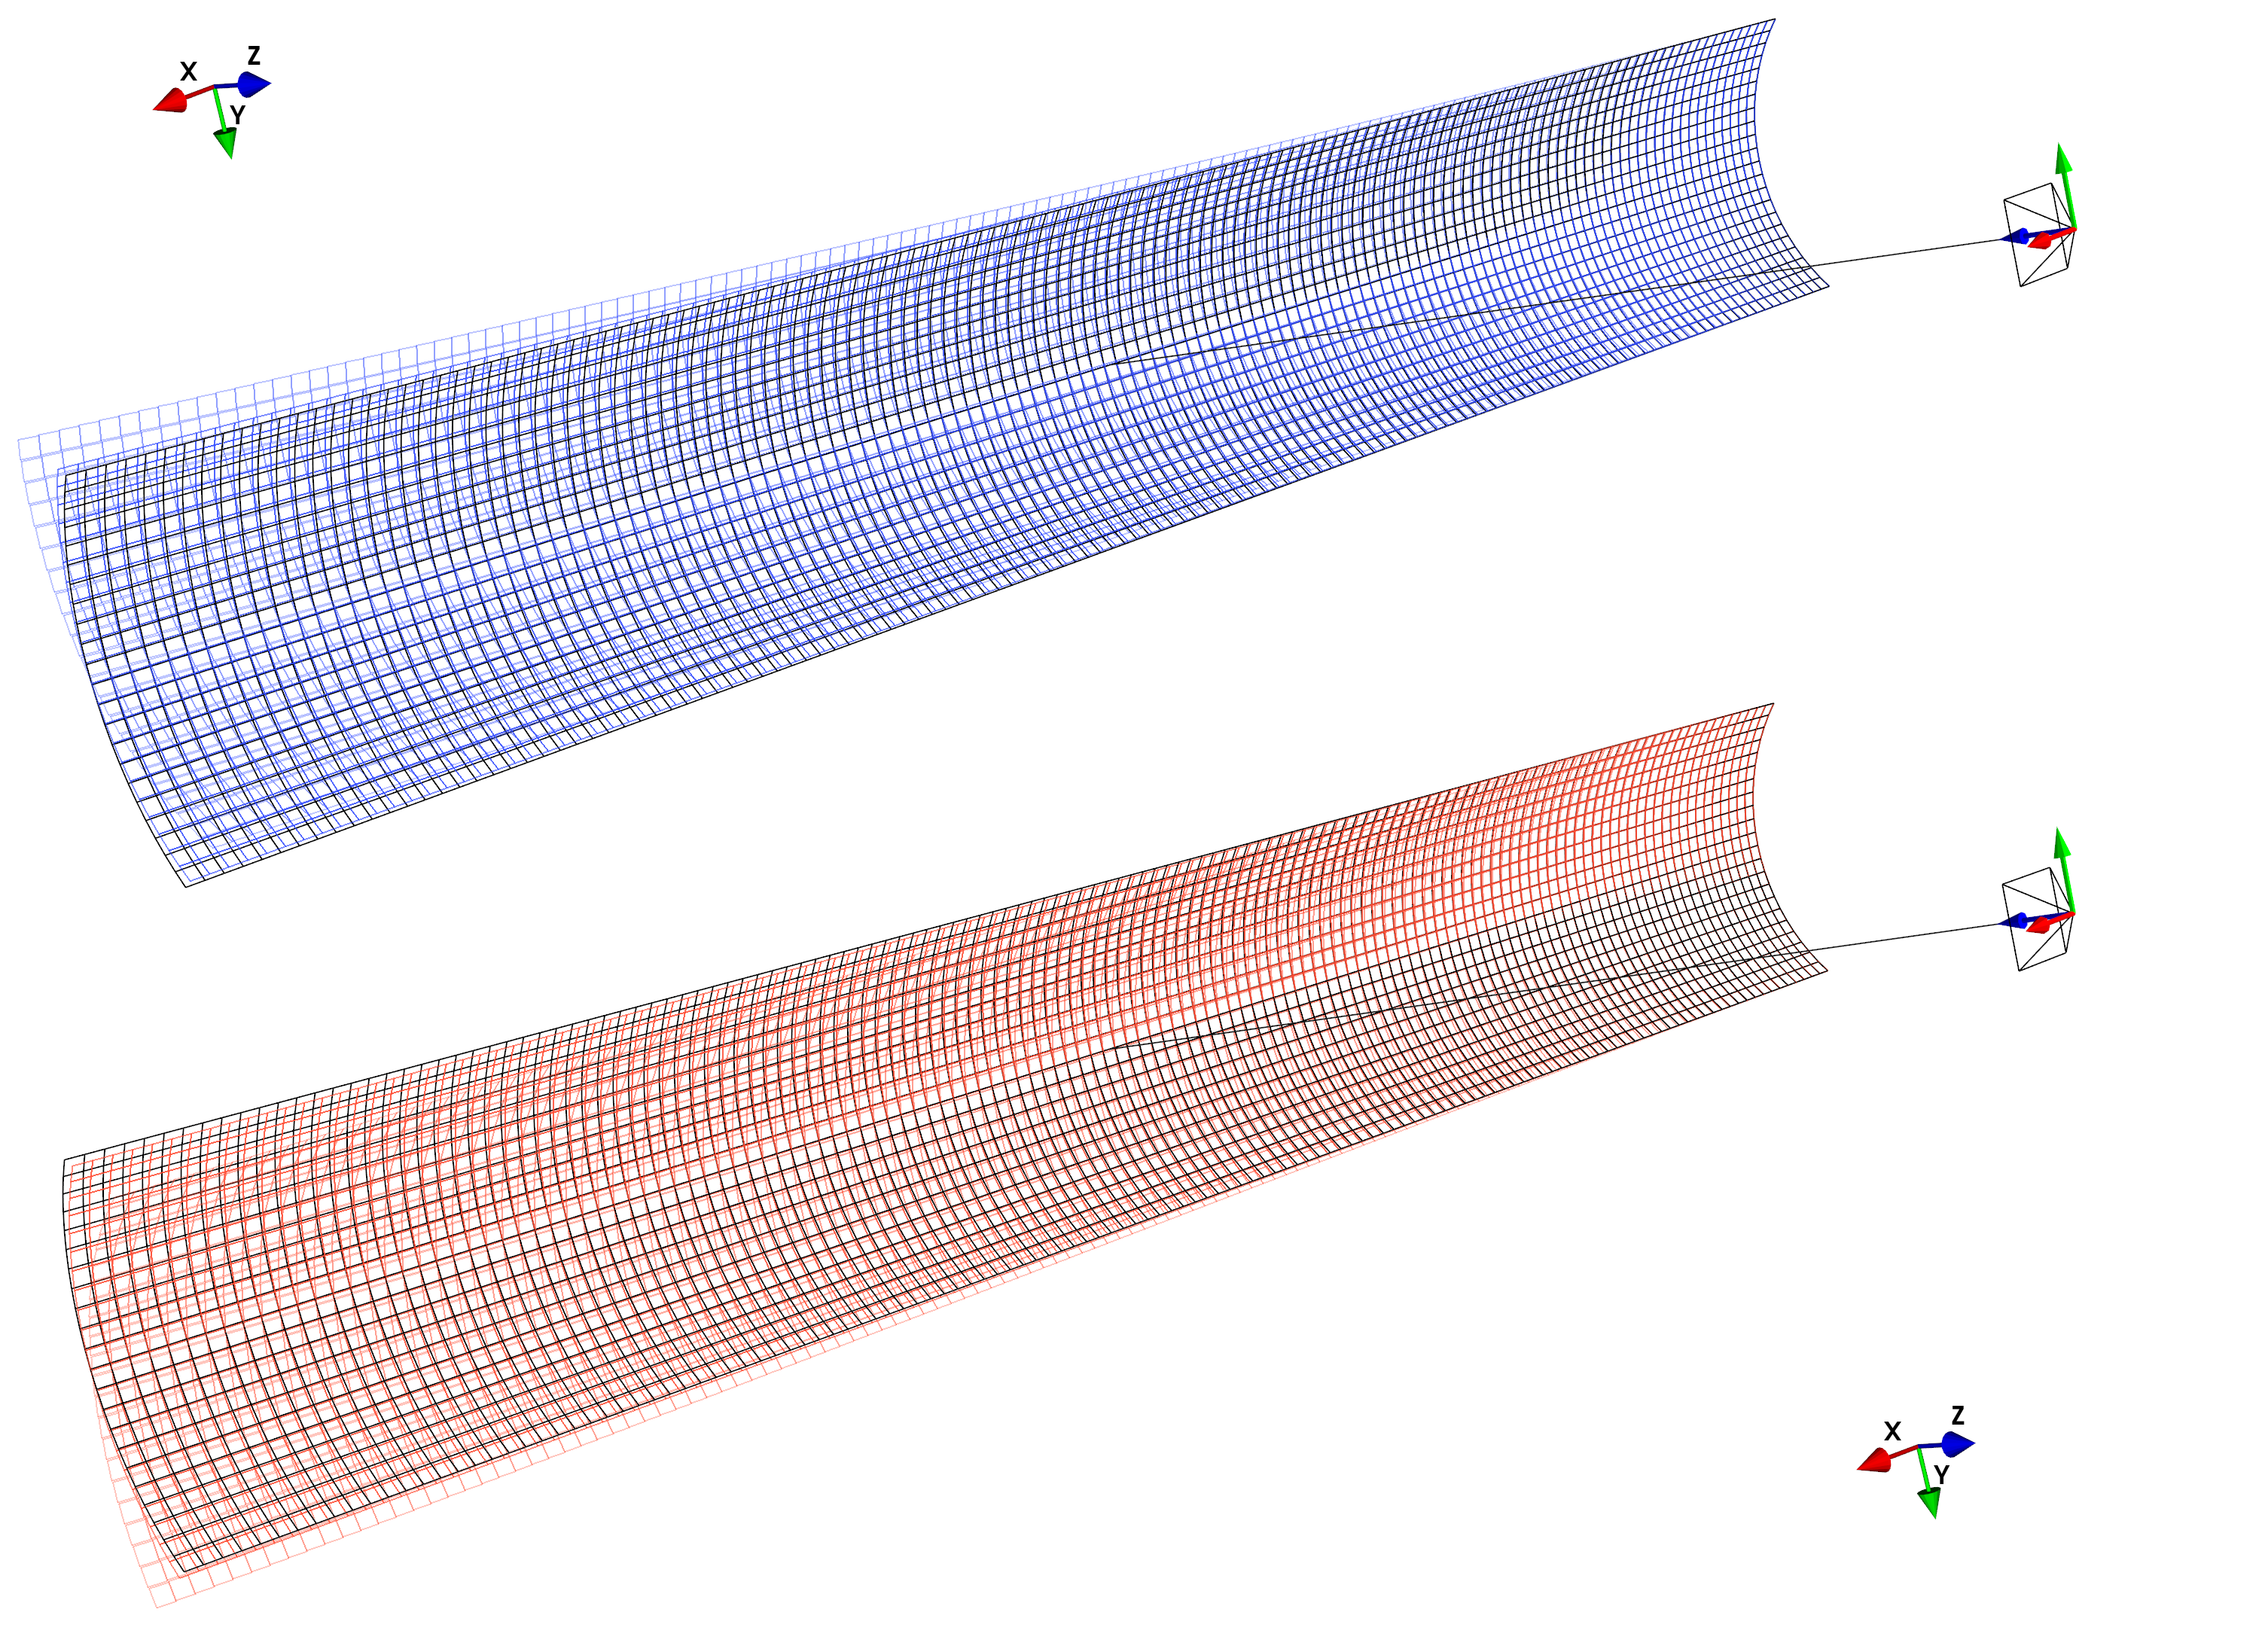
\includegraphics[width=\textwidth]{geometrydef}
        \caption{Reflectarray geometry under deformation( the deformation is exaggerated for visualization purposes.)}
        \label{fig:radef}
    \end{figure}
    The antennna pattern has an odd symmetry with respect to the oscillation phase $\varphi$ if the antenna structure is
    symmetrical with respect to the x or y axis and the modal deformation follows the same symmetry.
    In this case the deformation for positve and negative oscillation phases is symmetrical about the x-z plane, see Fig.~\ref{fig:radef};
    and, as a result, the antenna pattern is oddly symmetrical about the x-z plane relatively to the oscillation phase
    as visible in Figs.~\ref{fig:deformpattern} and~\ref{fig:deformpatternneg}.
    If the oscillation mode doesn't have an x or y axial symmetry, or the antenna structure is not symmetrical about the
    same plane (e.g., for the current scenatio if the feed is not on the x-z plane, see Fig.~\ref{fig:rageom}),
    the pattern symmetry is lost.


    \section{SAR Model}
    \label{sec:sar_model}

    \subsection{Geometrical and Stationary Phase Transformations}
    \label{subsec:transformations}
    write the relevant equations here
    \begin{figure}[!htb]
        \import{./figures}{pattern.pgf}
        \caption{Dynamic pattern (for oscillation frequency $f_{osc}=$2.78879~Hz, scene center oscillation phase
            $\varphi_0=0$, and relative amplitude 1) compared to the static pattern (right). In the Range-Doppler domain,
            for a broadside incidence angle of 17.3\degrees over the full illumination cone (horizon to horizon).
            The color scale is in dB.}
        \label{fig:RDpattern}
    \end{figure}

    \subsection{Ambiguity, SNR, and Pd with Dynamic Antenna Pattern}
    \label{subsec:ambiguity_snr_pd_with_dynamic_antenna_pattern}
    equations and plots of the range-Doppler space
    \begin{figure}[!htb]
        \import{./figures}{aasr_pattern.pgf}
        \caption{Detail of the static and dynamic patterns showing the integration domain for the AASR equation, main and ambiguous
        Doppler regions are marked by dashed lines. The color scale is in dB.
        }
        \label{fig:aasrpattern}
    \end{figure}
    \begin{figure}[!htb]
        \import{./figures}{aasr.pgf}
        \caption{AASR integrands (a) for initial oscillation phase $\varphi_0=0$, and computed AASR (b) for different $\varphi_0=0$ on different range cuts.
        }
        \label{fig:aasr}
    \end{figure}
    \begin{figure}[!htb]
        \import{./figures}{rasr_pattern.pgf}
        \caption{Detail of the static and dynamic patterns showing the integration domain for the RASR equation, main and ambiguous
        Range regions are marked by dashed lines. The color scale is in dB.
        }
        \label{fig:rasrpattern}
    \end{figure}
    \begin{figure}[!htb]
        \import{./figures}{rasr.pgf}
        \caption{RASR sum contributions~(a) for initial oscillation phase $\varphi_0=0$, and computed RASR~(b) for different $\varphi_0=0$ over visible range.
        }
        \label{fig:rasr}
    \end{figure}

    \subsection{Unambiguous Mode Design Point}
    \label{subsec:unambiguous_mode_design_point}
    algorithm and plots of the results\\
    \begin{figure}[!htb]
        \centering
        \import{./figures}{td_diagram_unamb.pgf}
        \caption{Unambiguous mode design point in the time diagram.
        }
        \label{fig:unambigmode}
    \end{figure}
    \FloatBarrier
    \noindent\rule{\textwidth}{0.4pt}
    \begin{ttfamily}
        \small
        Provided the maximum acceptable AASR and RASR,\\
        After findign the visible swath from the time diagram \\(knkowing PRF, approximate incidence angle and duty cycle):
        \begin{enumerate}
            \item Optimize looking angle to have same SNR at the shath extremes.
            \item Compute AASR in nominal case for a set of Doppler undersampling factors.
            \item \textbf{OR} Optimize the Doppler undersampling factor to lower AASR to AASR$_{\text{max}}$
            \item \textbf{IF} AASR nominal can be lowered to AASR$_{\text{max}}$
            \begin{enumerate}
                \item record optimal Bd
                \item Compute AASR for dynamic pattern for a set of mechanical \\oscillation $\varphi_0$, amplitudes and frequencies.
                \item Compute RASR in the static case
                \item Threshold RASR to RASR$_{\text{max}}$ and record the range values exceeding the threshold.
                \item Compute unambiguous swath
                \item \textbf{IF} unambiguous swath > 0
                \begin{enumerate}
                    \item Compute RASR for dynamic pattern for a set of \\mechanical oscillation $\varphi_0$, amplitudes and frequencies.
                \end{enumerate}
            \end{enumerate}
            \item compute SNR (static and dynamic) for the optimal Bd or the nominal Bd if no optimal is found
        \end{enumerate}
    \end{ttfamily}

    * to be expanded *\\
    \noindent\rule{\textwidth}{0.4pt}

    \begin{figure}[!htb]
        \centering
        \import{./figures}{results_unamb_legend.pgf}
        \import{./figures}{results_unamb.pgf}
        \caption{point map Unambiguous.}
        \label{fig:unambigresult}
    \end{figure}

    \subsection{Ambiguous Mode Design Point}
    \label{subsec:ambiguous_mode_design_point}
    algorithm and plots of the results
    \begin{figure}[!htb]
        \centering
        \import{./figures}{td_diagram_amb.pgf}
        \caption{Ambiguous mode design point in the time diagram.
        }
        \label{fig:ambigmode}
    \end{figure}

    \FloatBarrier
    \noindent\rule{\textwidth}{0.4pt}
    \begin{ttfamily}
        \small
        Provided the maximum acceptable RASR, the minimum acceptable probability of detection Pd$_{\text{min}}$;
        and all the radar parameters: power, bandwidth, noise figure + losses, probability of false alarm, ship area.\\
        After findign the visible swath from the time diagram \\(knkowing PRF, approximate incidence angle and duty cycle):
        \begin{enumerate}
            \item Optimize looking angle to have same Pd at the shath extremes.
            \item Compute the nominal Doppler bandwidth Bd from antenna length.
            \item Compute RASR in nominal case.
            \item Threshold RASR to RASR$_{\text{max}}$ and record the range values exceeding the threshold.
            \item Compute unambiguous swath
            \item \textbf{IF} unambiguous swath > 0
            \begin{enumerate}
                \item Compute RASR for dynamic pattern for a set of \\mechanical oscillation $\varphi_0$, amplitudes and frequencies.
                \item Compute AASR static and dynamic.
            \end{enumerate}
            \item Compute Pd and NESZ for the nominal (static) case.
            \item Find usable Pd swath (where Pd > Pd$_{\text{min}}$)
            \item \textbf{IF} usable Pd swath > 0
            \begin{enumerate}
                \item Compute Pd and NESZ for the dynamic case (for a set of amplitudes, freq and phases).
            \end{enumerate}
            \item \textbf{Return} all the results
        \end{enumerate}
    \end{ttfamily}

    * to be expanded *\\
    \noindent\rule{\textwidth}{0.4pt}

    \begin{figure}[!htb]
        \centering
        \import{./figures}{results_amb_legend.pgf}
        \import{./figures}{results_amb.pgf}
        \caption{point map Ship Detection.}
        \label{fig:ambigresult}
    \end{figure}

    \subsection{Design Space Mapping}
    \label{subsec:design_space_mapping}

    \subsection{Worsening due to oscillation metrics}
    \label{subsec:worsening_due_to_oscillation_metrics}
    TBD


%% Bibliography
    \bibliographystyle{ieeetr}
    \bibliography{../src/main.bib}

    textwidth in pt: \the\textwidth \\
    textwidth in cm: \printinunitsof{cm}\prntlen{\textwidth}\\
    textwidth in inch: \printinunitsof{in}\prntlen{\textwidth}\\


\end{document}
